%%%%%%%%%%%%%%%%%%%%%%%%%%%%%%%%%%%%%%%%%
% Beamer Presentation
% LaTeX Template
% Version 1.0 (10/11/12)
%
% This template has been downloaded from:
% http://www.LaTeXTemplates.com
%
% License:
% CC BY-NC-SA 3.0 (http://creativecommons.org/licenses/by-nc-sa/3.0/)
%
%%%%%%%%%%%%%%%%%%%%%%%%%%%%%%%%%%%%%%%%%

%----------------------------------------------------------------------------------------
%	PACKAGES AND THEMES
%----------------------------------------------------------------------------------------

\documentclass{beamer}
\usepackage{xcolor}
\usepackage{graphicx}
\usepackage{tikz}
\usepackage{listings}
\usepackage{multicol}

\definecolor{applegreen}{rgb}{0.55, 0.71, 0.0}
\definecolor{blue(ncs)}{rgb}{0.0, 0.45, 0.60}
\definecolor{burgundy}{rgb}{0.5, 0.0, 0.13}

\definecolor{cadet}{rgb}{0.33, 0.41, 0.47}
\definecolor{airforceblue}{rgb}{0.36, 0.54, 0.66}

\lstdefinestyle{C}{
  language=C,
  emptylines=1,
  breaklines=true,
  basicstyle=\ttfamily\color{black},
  identifierstyle=\ttfamily,
  keywordstyle=\color[rgb]{0.0, 0.0, 1.0},
  stringstyle=\color[rgb]{1.0, 0.0, 0.0},
  commentstyle=\color{gray}\slshape,
}

\lstdefinestyle{assembly}{
  emptylines=1,
  breaklines=true,
  basicstyle=\ttfamily\color{black},
  identifierstyle=\ttfamily,
  keywordstyle=\color[rgb]{1.0, 0.0, 1.0},
  stringstyle=\color[rgb]{1.0, 0.0, 0.0},
  commentstyle=\color{gray}\slshape,
  morekeywords={vmovapd, vfmadd231pd,vfnmadd213pd, vmulpd},
}

\lstdefinestyle{qfunc}{
  language=C,
  emptylines=1,
  breaklines=true,
  basicstyle=\ttfamily\color{black},
  commentstyle=\color{gray}\slshape,
  moredelim=**[is][\color{applegreen}]{@}{@},
  moredelim=**[is][\color{blue(ncs)}]{!}{!},
  moredelim=**[is][\color{green!40!black}]{z}{z},
  moredelim=**[is][\color{blue(ncs)!80}]{#}{#},
  moredelim=**[is][\color{blue(ncs)!80!black}]{'}{'},
}

\lstdefinestyle{oper}{
  language=C,
  emptylines=1,
  breaklines=true,
  basicstyle=\ttfamily\color{black},
  moredelim=**[is][\color{applegreen}]{@}{@},
  moredelim=**[is][\color{blue(ncs)}]{!}{!},
  moredelim=**[is][\color{burgundy}]{#}{#},
  moredelim=**[is][\color{red}]{'}{'},
  moredelim=**[is][\bf]{z}{z},
}

\mode<presentation> {

\usetheme{CambridgeUS}

\usecolortheme{wolverine}

\definecolor{gold}{HTML}{D4A017}
\definecolor{darkgold}{HTML}{B7950B}

\setbeamercolor{palette primary}{bg=cadet,fg=white}
\setbeamercolor{palette secondary}{bg=airforceblue,fg=white}
\setbeamercolor{palette tertiary}{bg=black,fg=white}
\setbeamercolor{palette quaternary}{bg=cadet,fg=white}

\setbeamercolor{frametitle}{bg=airforceblue,fg=white}

\setbeamercolor{section number projected}{bg=black,fg=cadet}
\setbeamercolor{item}{fg=black,bg=cadet}

\setbeamertemplate{page number in head/foot}[framenumber]
}

\usepackage{graphicx} % Allows including images
\usepackage{booktabs} % Allows the use of \toprule, \midrule and \bottomrule in tables

%----------------------------------------------------------------------------------------
%	TITLE PAGE
%----------------------------------------------------------------------------------------

\title[libCEED Finite Element Library]{Matrix Free Multigrid with libCEED\\Challenges and Applications} % The short title appears at the bottom of every slide, the full title is only on the title page

\author[Jeremy L Thompson]{Jeremy L Thompson} % Your name
\institute[CU Boulder] % Your institution as it will appear on the bottom of every slide, may be shorthand to save space
{University of Colorado Boulder \\ % Your institution for the title page
\medskip
\textit{jeremy.thompson@colorado.edu} % Your email address
}
\date{Sept 27, 2019} % Date, can be changed to a custom date

\begin{document}

\begin{frame}
\titlepage % Print the title page as the first slide
\end{frame}

%------------------------------------------------

\begin{frame}
\begin{center}
\frametitle{libCEED Team}

{\flushleft

Developers: \hspace{2mm} Jed Brown\textsuperscript{1}, Jeremy Thompson\textsuperscript{1} \\
\hspace{23mm}  Thilina Rathnayake\textsuperscript{2}, Jean-Sylvain Camier\textsuperscript{3}, Tzanio Kolev\textsuperscript{3},\\
\hspace{23mm} Veselin Dobrev\textsuperscript{3}, Valeria Barra\textsuperscript{1}, Yohann Doudouit\textsuperscript{3},\\
\hspace{23mm} David Medina\textsuperscript{4}, Tim Warburton\textsuperscript{5}, \& Oana Marin\textsuperscript{6}\\

~\\

Grant: \hspace{11mm} Exascale Computing Project (17-SC-20-SC)\\

~\\

~\\

\small{1: University of Colorado, Boulder\\
2: University of Illinois, Urbana-Champaign\\
3: Lawrence Livermore National Laboratory\\
4: OCCA\\
5: Virginia Polytechnic Institute and State University\\
6: Argonne National Laboratory\\}}

\end{center}
\end{frame}

\begin{frame}
\begin{center}
\frametitle{Overview}

libCEED is an extensible library that provides a portable algebraic\\
interface and optimized implementations of high-order operators\\

~\\

~\\

libCEED finite element operator decomposition provides opportunities\\for optimization and smart preconditioning\\

~\\

~\\

P-multigrid example offers insights into more flexible\\preconditioning techniques

\end{center}
\end{frame}
 
%------------------------------------------------

\begin{frame}
\frametitle{Overview} % Table of contents slide, comment this block out to remove it
\tableofcontents % Throughout your presentation, if you choose to use \section{} and \subsection{} commands, these will automatically be printed on this slide as an overview of your presentation
\end{frame}

%----------------------------------------------------------------------------------------
%	PRESENTATION SLIDES
%----------------------------------------------------------------------------------------

%------------------------------------------------
\section{Introduction}
%------------------------------------------------

\begin{frame}
\begin{center}
\frametitle{Center for Efficient Exascale Discretizations}

\begin{flushleft}
DoE exascale co-design center\\

~\\
\end{flushleft}

\begin{itemize}

\item Design discretization algorithms for exascale hardware that deliver significant performance gain over low order methods\\

~\\

\item Collaborate with hardware vendors and software projects for exascale hardware and software stack\\

~\\

\item Provide efficient and user-friendly unstructured PDE discretization component for exascale software ecosystem

\end{itemize}

\end{center}
\end{frame}

%------------------------------------------------

\begin{frame}
\begin{center}
\frametitle{Tensor Product Elements}

\setlength{\columnsep}{15mm}
\begin{multicols}{2}

\begin{flushright}
\includegraphics[height=5cm]{libCEEDAssembledVsTensorApply}
\end{flushright}

\begin{flushleft}
\includegraphics[height=5cm]{libCEEDAssembledVsTensorStorage}
\end{flushleft}

\end{multicols}

Using an assembled matrix forgoes performance optimizations\\
for hexahedral elements

\end{center}
\end{frame}

%------------------------------------------------
\section{libCEED}
%------------------------------------------------

%------------------------------------------------

\begin{frame}
\begin{center}
\frametitle{libCEED Design}

libCEED design approach:\\

~\\

\begin{itemize}

\item Avoid global matrix assembly\\

~\\

\item Optimize basis operations for all architectures\\

~\\

\item Single source user quadrature point functions\\

~\\

\item Easy to parallelize across hetrogeneous nodes

\end{itemize}

\end{center}
\end{frame}

%------------------------------------------------

\begin{frame}
\begin{center}
\frametitle{libCEED Backends}

\includegraphics[height=6.5cm]{libCEEDBackends}

libCEED provides multiple backend implementations\\

\end{center}
\end{frame}

%------------------------------------------------

\begin{frame}
\begin{center}
\frametitle{libCEED Operator Decomposition}

\includegraphics[height=4.5cm]{libCEEDAPI}

\small{

\hspace{1.8cm}${\color{burgundy}A}_L = G^T {\color{blue(ncs)}B^T} {\color{applegreen}D} {\color{blue(ncs)}B} G$

\begin{itemize}

\item $G$ - CeedElemRestriction, local gather/scatter

\item {\color{blue(ncs)}$B$} - CeedBasis, provides basis operations such as interp and grad

\item {\color{applegreen}$D$} - CeedQFunction, representation of PDE at quadrature points

\item ${\color{burgundy}A}_L$ - CeedOperator, aggregation of Ceed objects for local action of operator

\end{itemize}

}

\end{center}
\end{frame}

%------------------------------------------------

\begin{frame}
\begin{center}
\frametitle{Laplacian Example}

Solving the 2D Poisson problem: $-\Delta u = f$\\

Weak Form: $\int \nabla v \nabla u = \int v f$\\
~\\

\begin{itemize}

\item General libCEED Operator

      ${\color{burgundy}A}_L = G^T {\color{blue(ncs)}B^T} {\color{applegreen}D} {\color{blue(ncs)}B} G$\\
~\\

\item Laplacian Operator

      ${\color{burgundy}A}_L = G^T {\color{blue(ncs)}B_{Grad2D}^T} {\color{applegreen}D} {\color{blue(ncs)}B_{Grad2D}} G$

\end{itemize}

where ${\color{applegreen}D}$ is block diagonal by quadrature point:\\
      ${\color{applegreen}D_i} = \left( w_i \det{J_{geo}}\right) J_{geo}^{-1} J_{geo}^{-T}$ and
      $J_{geo} = \left[ \begin{tabular}{cc}
$\frac{\partial x}{\partial r}$ & $\frac{\partial x}{\partial s}$\\
$\frac{\partial y}{\partial r}$ & $\frac{\partial y}{\partial s}$
\end{tabular} \right]$\\
      $x, y$ physical coords; $r, s$ reference coords

\end{center}
\end{frame}

%------------------------------------------------

\begin{frame}
\begin{center}
\frametitle{Basis Optimization}

Solving the 2D Poisson problem: $-\Delta u = f$\\

Weak Form: $\int \nabla v \nabla u = \int v f$\\
~\\

\begin{itemize}

\item General libCEED Operator

      ${\color{burgundy}A}_L = G^T {\color{blue(ncs)}B^T} {\color{applegreen}D} {\color{blue(ncs)}B} G$\\
~\\

\item Laplacian Operator

      ${\color{burgundy}A}_L = G^T {\color{blue(ncs)}B_{Grad2D}^T} {\color{applegreen}D} {\color{blue(ncs)}B_{Grad2D}} G$\\
~\\

\item Computationally Efficient Form

      ${\color{burgundy}A}_L = G^T {\color{blue(ncs)} \left[ \begin{tabular}{cc}
$B_{G}^T \otimes B_{I}^T$ & $B_{I}^T \otimes B_{G}^T$
\end{tabular} \right]} {\color{applegreen}D} {\color{blue(ncs)} \left[ \begin{tabular}{c}
$B_{G} \otimes B_{I}$\\
$B_{I} \otimes B_{G}$
\end{tabular} \right]} {\color{black} G}$\\
      ${\color{blue(ncs)}B_I}$ - $1$D Interpolation\\
      ${\color{blue(ncs)}B_G}$ - $1$D Gradient

\end{itemize}

\end{center}
\end{frame}

%------------------------------------------------

\begin{frame}
\begin{center}
\frametitle{Basis Optimization}

Solving the 2D Poisson problem: $-\Delta u = f$\\

Weak Form: $\int \nabla v \nabla u = \int v f$\\
~\\

\begin{itemize}

\item General libCEED Operator

      ${\color{burgundy}A}_L = G^T {\color{blue(ncs)}B^T} {\color{applegreen}D} {\color{blue(ncs)}B} G$\\
~\\

\item Laplacian Operator

      ${\color{burgundy}A}_L = G^T {\color{blue(ncs)}B_{Grad2D}^T} {\color{applegreen}D} {\color{blue(ncs)}B_{Grad2D}} G$\\
~\\

\item Computationally Efficient Form

      ${\color{burgundy}A}_L = G^T {\color{blue(ncs)} \left( B_{I}^T \otimes B_{I}^T \right) \left[ \begin{tabular}{cc}
$\hat{B}_{G}^T \otimes I_2$ & $I_2 \otimes \hat{B}_{G}^T$
\end{tabular} \right]} {\color{applegreen}D} {\color{blue(ncs)} \left[ \begin{tabular}{c}
$\hat{B}_{G} \otimes I_2$\\
$I_2 \otimes \hat{B}_{G}$
\end{tabular} \right] \left( B_{I} \otimes B_{I} \right)} {\color{black} G}$\\
    where ${\color{blue(ncs)}\hat{B}_{G} = B_{G} B_{I}}$

\end{itemize}

\end{center}
\end{frame}

%------------------------------------------------

\begin{frame}[fragile]
\begin{center}
\frametitle{Operator Definition}

General libCEED Operator:\\

${\color{red}v}_L = {\color{burgundy}A}_L {\color{red}u}_L$\\

~\\

${\color{burgundy}A}_L = {\bf G^T} {\color{blue(ncs)}B^T} {\color{applegreen}D} {\color{blue(ncs)}B} {\bf G}$\\

~\\~\\

Laplacian Operator Code:
{\scriptsize
\begin{lstlisting}[style=oper]
CeedOperatorCreate(ceed, @qf_apply@, NULL, NULL, &#op_apply#);
CeedOperatorSetField(#op_apply#, "du", zerestrictuz, CEED_TRANSPOSE,
                     !basisu!, 'CEED_VECTOR_ACTIVE');
CeedOperatorSetField(#op_apply#, "geo",erestrictqdi,CEED_NOTRANSPOSE,
                     !CEED_BASIS_COLLOCATED!, geo);
CeedOperatorSetField(#op_apply#, "dv", zerestrictuz, CEED_TRANSPOSE,
                     !basisu!, 'CEED_VECTOR_ACTIVE');
...
CeedOperatorApply(#op_apply#, 'uloc', 'vloc', CEED_REQUEST_IMMEDIATE);
\end{lstlisting}
}

\end{center}
\end{frame}

%------------------------------------------------

\begin{frame}[fragile]
\begin{center}
\frametitle{QFunction Definition}

General libCEED QFunction:\\

${\color{blue(ncs)!80!black}v_q} = {\color{applegreen}D} {\color{blue(ncs)!80}u_q}$\\

~\\

2D Laplacian QFunction:\\

${\color{blue(ncs)}\left[} {\color{blue(ncs)!80!black} \begin{tabular}{c}
$dv_0$\\ $dv_1$ \end{tabular}} {\color{blue(ncs)}\right]} = {\color{applegreen} \left[} {\color{green!40!black} \begin{tabular}{cc}
$D_{00}$ & $D_{01}$\\
$D_{01}$ & $ D_{11}$ \end{tabular}} {\color{applegreen}\right]} {\color{blue(ncs)}\left[} {\color{blue(ncs)!80} \begin{tabular}{c}
$du_0$\\ $du_1$ \end{tabular} } {\color{blue(ncs)}\right]}$\\

~\\

~\\

2D Laplacian QFunction Code:
{\scriptsize
\begin{lstlisting}[style=qfunc]
CeedQFunctionCreateInterior(ceed, 1, Poisson2D,
                            Poisson2D_loc, &@qf_apply@);
CeedQFunctionAddInput(@qf_apply@, #"du"#, 2, !CEED_EVAL_GRAD!);
CeedQFunctionAddInput(@qf_apply@, z"geo"z, 3, CEED_EVAL_NONE);
CeedQFunctionAddOutput(@qf_apply@, '"dv"', 2, !CEED_EVAL_GRAD!);
\end{lstlisting}
}

\end{center}
\end{frame}

%------------------------------------------------

\begin{frame}[fragile]
\begin{center}
\frametitle{QFunction Definition}

\begin{itemize}

\item Single Source QFunctions for all backends:\\

~\\

\item C/C++ code, compiled with main for CPU, JiT for GPU\\

\end{itemize}

~\\

{\scriptsize
\begin{lstlisting}[style=qfunc]
int Poisson2D(void *ctx, const CeedInt Q,
    const CeedScalar *const *in, CeedScalar *const *out) {
  // Inputs and Outputs
  const CeedScalar #*du# = in[0];
  CeedScalar z*geoz = out[0], '*dv' = out[1];

  // Quadrature Point Loop
  CeedPragmaSIMD // For CPU vectorization
  for (CeedInt i=0; i<Q; i++) {
    'dv[i+Q*0]' = zgeo[i+Q*0]z*#du[i+Q*0]# + zgeo[i+Q*2]z*#du[i+Q*1]#;
    'dv[i+Q*1]' = zgeo[i+Q*2]z*#du[i+Q*0]# + zgeo[i+Q*1]z*#du[i+Q*1]#;
  } // End of Quadrature Point Loop

  return 0;
}
\end{lstlisting}
}

\end{center}
\end{frame}

%------------------------------------------------
\section{P-Multigrid}
%------------------------------------------------

\begin{frame}
\begin{center}
\frametitle{P-Multigrid}

\begin{itemize}

\item Preconditioning essential for iterative solvers, especially with high order\\

~\\

\item Multigrid preconditioning offers $O(N)$ elliptic PDE solve\\

~\\

\item H-multigrid difficult on unstructured/mixed meshes

\end{itemize}

\end{center}
\end{frame}

%------------------------------------------------

\begin{frame}
\begin{center}
\frametitle{V-Cycle}

3 level multigrid example\\
~\\

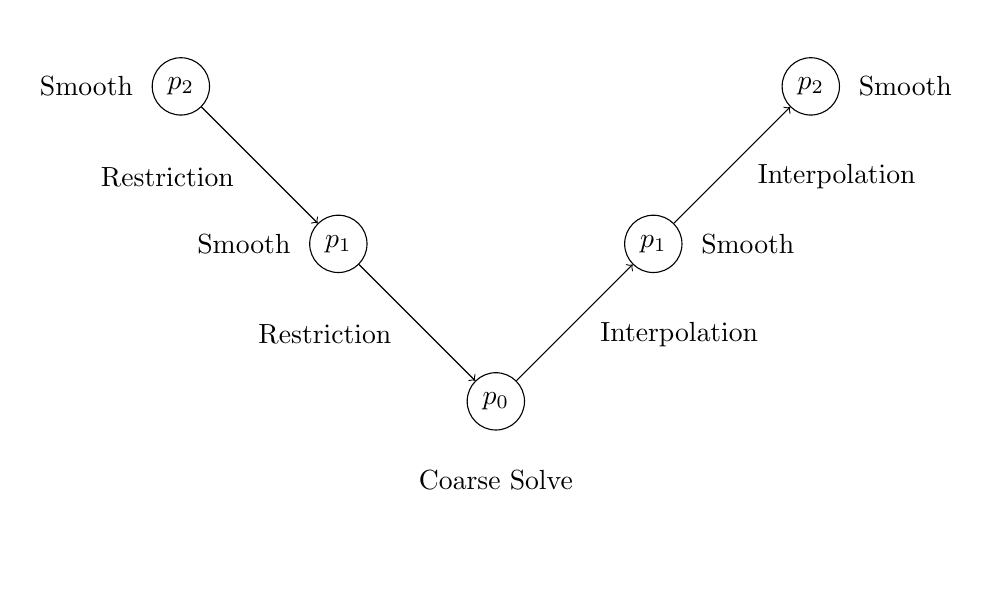
\begin{tikzpicture}
\node[shape=circle,draw=black] (A) at (0,0) {$p_2$};
\node[shape=circle] (Al) at (-1.2,0) {Smooth};
\node[shape=circle,draw=black] (B) at (2,-2) {$p_1$};
\node[shape=circle] (Bl) at (0.8,-2) {Smooth};
\node[shape=circle,draw=black] (C) at (4,-4) {$p_0$};
\node[shape=circle] (Cl) at (4,-5) {Coarse Solve};
\node[shape=circle,draw=black] (D) at (6,-2) {$p_1$};
\node[shape=circle] (Dl) at (7.2,-2) {Smooth};
\node[shape=circle,draw=black] (E) at (8,0) {$p_2$};
\node[shape=circle] (El) at (9.2,0) {Smooth};
\path[->] (A) edge node[left=10, pos=.6] {Restriction} (B);
\path[->] (B) edge node[left=10, pos=.6] {Restriction} (C);
\path[->] (C) edge node[right=10, pos=.4] {Interpolation} (D);
\path[->] (D) edge node[right=10, pos=.4] {Interpolation} (E);
\end{tikzpicture}

\end{center}
\end{frame}

%------------------------------------------------

\begin{frame}
\begin{center}
\frametitle{libCEED Operators - Laplacian}

Solving the 2D Poisson problem: $-\Delta u = f$\\

Weak Form: $\int \nabla v \nabla u = \int v f$\\
~\\

\begin{itemize}

\item General libCEED Operator

      ${\color{burgundy}A}_L = G^T {\color{blue(ncs)}B^T} {\color{applegreen}D} {\color{blue(ncs)}B} G$\\
~\\

\item Laplacian Operator

      ${\color{burgundy}A}_L = G^T {\color{blue(ncs)}B_{Grad2D}^T} {\color{applegreen}D} {\color{blue(ncs)}B_{Grad2D}} G$\\
~\\

\item Computationally Efficient Form

      ${\color{burgundy}A}_L = G^T {\color{blue(ncs)} \left( B_{I}^T \otimes B_{I}^T \right) \left[ \begin{tabular}{cc}
$\hat{B}_{G}^T \otimes I_2$ & $I_2 \otimes \hat{B}_{G}^T$
\end{tabular} \right]} {\color{applegreen}D} {\color{blue(ncs)} \left[ \begin{tabular}{c}
$\hat{B}_{G} \otimes I_2$\\
$I_2 \otimes \hat{B}_{G}$
\end{tabular} \right] \left( B_{I} \otimes B_{I} \right)} {\color{black} G}$\\
    where ${\color{blue(ncs)}\hat{B}_{G} = B_{G} B_{I}}$

\end{itemize}

\end{center}
\end{frame}

%------------------------------------------------

\begin{frame}
\begin{center}
\frametitle{libCEED Operators - Restriction}

Restriction / Interpolation is largely a basis operation\\
~\\

\begin{itemize}

\item General libCEED Operator

${\color{burgundy}A}_L = G^T {\color{blue(ncs)}B^T} {\color{applegreen}D} {\color{blue(ncs)}B} G$\\
~\\

\item Restriction / Interpolation Operator

${\color{burgundy}A}_L = G_c^T {\color{blue(ncs)}I} {\color{applegreen}I} {\color{blue(ncs)}B_{f to c}} G_f$\\
~\\

\item Computationaly Efficient Form

${\color{burgundy}A}_L = G_c^T {\color{blue(ncs)}\left( \hat{J}_{f to c} \otimes \hat{J}_{f to c} \right)} G_f$

\end{itemize}

\end{center}
\end{frame}

%------------------------------------------------

\begin{frame}
\begin{center}
\frametitle{Performance}

\begin{itemize}

\item $3$D Poisson Problem\\

~\\

\item Small test on personal laptop\\

~\\

\item Mesh

\begin{itemize}

\item $8^3$ GLL points per element

\item Quadrature on $9^3$ GL points per element

\item Cube with $32^3$ elements, $89,200$ DoFs

\end{itemize}

\end{itemize}

{\small

\setlength\columnsep{1pt}

\begin{multicols}{2}

\begin{itemize}

\setlength{\leftmarginii}{1em}

\item Unpreconditioned

\begin{itemize}

\item 9.916e-06 \hfill $\lvert \lvert \cdot \rvert \rvert_\infty$ Error \hspace{1em}

\item $306$ \hfill CG iterations \hspace{1em}

\item 11.838 million \hfill CG DoFs/sec \hspace{1em}

\item 2.306 sec \hfill CG solve time \hspace{1em}

\end{itemize}

\item P-Multigrid

\begin{itemize}

\item 9.916e-06 \hfill $\lvert \lvert \cdot \rvert \rvert_\infty$ Error \hspace{1em}

\item $59$ \hfill CG iterations \hspace{1em}

\item 0.3211 million \hfill CG DoFs/sec \hspace{1em}

\item 16.390 sec \hfill CG solve time \hspace{1em}

\end{itemize}

\end{itemize}

\end{multicols}

}

\end{center}
\end{frame}

%------------------------------------------------

\begin{frame}
\begin{center}
\frametitle{Challenges}

\begin{itemize}

\item Significantly decreased number of iterations... but\\

~\\

\begin{itemize}

\item Iterations much slower than desired\\

~\\

\item Can decrease iteration time with lighter smoother\\

~\\

\item High order requires more levels, increased communication\\

\end{itemize}

~\\

\item Caveats:

\begin{itemize}

\item Small mesh run for demo purposes\\

~\\

\item PETSc code currently has issues running with CUDA in parallel

\end{itemize}

\end{itemize}

\end{center}
\end{frame}

%------------------------------------------------
\section{Current Efforts}
%------------------------------------------------

\begin{frame}
\begin{center}
\frametitle{Way Forward}

\begin{itemize}

\item Balancing Domain Decomposition by Constraints\\

~\\

\item Designed for partially subassembled finite element operators\\

~\\

\item Two levels, primal constraints and full mesh\\

~\\

\item Lower communication, but heavier smoother required\\

\end{itemize}

\end{center}
\end{frame}
%------------------------------------------------

\begin{frame}
\begin{center}
\frametitle{Inexact Subdomain Solves}

\begin{itemize}

\item Inexact subdomain solves (Li and Widlund 2007)\\

~\\

\item Fast Diagonalization for inverses of separable operators\\
      - Used in some Additive Schwartz methods (Nek5000)\\

~\\

\item Fast Diagonalization Method inspired subdomain approximate inverses\\

\end{itemize}

\includegraphics[height=4.0cm]{BDDCInexactSolves}

\end{center}
\end{frame}

%------------------------------------------------
\section{Future Work}
%------------------------------------------------

\begin{frame}
\begin{center}
\frametitle{Future Work}

\begin{itemize}

\item Further performance enhancements (GPU and CPU)\\

~\\

\item Improved mixed mesh and operator composition support\\

~\\

\item Expanded non-linear and multi-physics examples\\

~\\

\item Preconditioning based on libCEED operator decomposition\\

~\\

\item Algorithmic differentiation of user quadrature functions\\

~\\

\item We invite contributors and friendly users

\end{itemize}

\end{center}
\end{frame}

%------------------------------------------------
\section{Questions}
%------------------------------------------------

\begin{frame}
\begin{center}
\frametitle{Questions?}

{\flushleft

Advisors : \hspace{5mm} Jed Brown\textsuperscript{1} \& Daniel Appel\"{o}\textsuperscript{1}\\

~\\

Collaborators: Valeria Barra\textsuperscript{1}, Oana Marin\textsuperscript{2}, Tzanio Kolev\textsuperscript{3},\\
\hspace{23mm} Jean-Sylvain Camier\textsuperscript{3}, Veselin Dobrev\textsuperscript{3}, Yohann Doudouit\textsuperscript{3},\\
\hspace{23mm} Tim Warburton\textsuperscript{4}, David Medina\textsuperscript{5}, \& Thilina Rathnayake\textsuperscript{6}\\

~\\

Grant: \hspace{11mm} Exascale Computing Project (17-SC-20-SC)\\

~\\

~\\

\small{1: University of Colorado, Boulder\\
2: Argonne National Laboratory\\
3: Lawrence Livermore National Laboratory\\
4: Virginia Polytechnic Institute and State University\\
5: OCCA\\
6: University of Illinois, Urbana-Champaign\\}}

\end{center}
\end{frame}

%------------------------------------------------

\begin{frame}[noframenumbering]
\titlepage % Print the title page
\end{frame}

%------------------------------------------------

%----------------------------------------------------------------------------------------

\end{document}

